\documentclass{article}
\usepackage{amsmath,amssymb,setspace,verbatim,graphicx,enumerate,enumitem}
\usepackage[top=1in,bottom=1in,left=1in,right=1in,nohead,nofoot]{geometry}
\usepackage{caption}
% \usepackage{subcaption}
\usepackage{subfig}
% \usepackage{subfloat}
\usepackage{tabularx}
\usepackage{mdframed}

\newenvironment{Rcode}% environment name 
{%begin code
    \begin{mdframed}
    \#R code
    \begin{small}
}
{%end code
    \end{small}
    \end{mdframed}
}

\newenvironment{console}% environment name 
{%begin code
    \begin{mdframed}
    \#Console
    \begin{small}
}
{%end code
    \end{small}
    \end{mdframed}
}

% \parindent 0in
% \parskip .2in
% \pagestyle{empty} \singlespacing
% %\newcommand{\vect}[1]{\mbox{\boldmath $ #1$}}
% \newcommand{\bv}[1]{\mathbf{#1}}
% \setlist{noitemsep,topsep=0pt,parsep=0pt,partopsep=0pt}


\begin{document}
\title{FDA Homework 1}
\author{Seokjun Choi}
\date{September 30, 2019}
\maketitle

\section{Chapter 1}
\subsection{Problem 1}

The pinch is a dataset included in the fda package. It consists of 151 measurements of pinch force for 20 replications (curves). 

\subsubsection*{(a)  Convert the pinch data to functional objects using 15 B-splines of order four (cubic splines) and plot the 20 smoothed curves on one graph.}
To get the result we want, call the fda package and execute the code below.

\begin{Rcode}
    \begin{verbatim}
b_spline_basis<-create.bspline.basis(c(1,151), nbasis=15)
pinch.F<-Data2fd(1:151, pinch, b_spline_basis)
plot(pinch.F)
    \end{verbatim}
\end{Rcode}
Then we get the result.
\begin{figure}[hh]
    \centering
    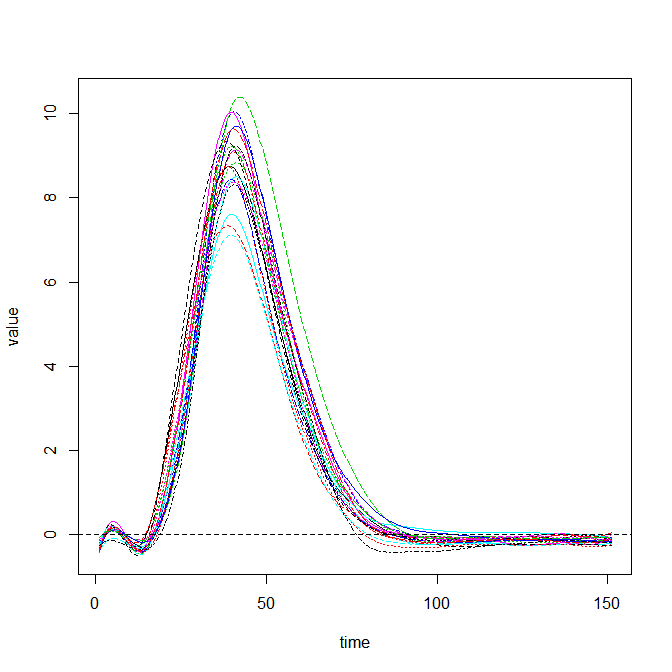
\includegraphics[height=8cm]{pinch_F_plot.png}
    \caption{fitting pinch data using 15 b-splines}
\end{figure}

\newpage
\subsubsection*{(b) Calculate the pointwise mean and SD and add them to the plot.}
For calculation, run the code below.
\begin{Rcode}
    \begin{verbatim}
pinch.F.mean <- mean(pinch.F)
pinch.F.mean$coefs

pinch.F.std <- std.fd(pinch.F)
pinch.F.std$coefs

par(mar=c(4,4,1,1))
plot(pinch.F, col="grey")
plot(pinch.F.mean,lwd=4,add=TRUE)
plot(pinch.F.std, lwd=4, add=TRUE, col="red")
    \end{verbatim}
\end{Rcode}

For analytic expression of pointwise mean and point sd, denote $b_i$ as i-th b-spline of order 4
on domain $[0,120] \subset \Re$. Then
\[Mean(x)=\sum_{i=1}^{16}c_ib_i(x)\]
\[Sd(x)=\sum_{i=1}^{16}s_ib_i(x)\]
where $c_i$ : -0.31109576, 0.73142704, -1.63349675, 2.72475346, 10.93667264, 6.03218354, 2.28791198, 0.34957598, -0.09607592, -0.16637125, -0.11240041, -0.15664938, -0.10293668, -0.16311715, -0.11897440
and $s_i$ : 0.0846463, 0.1182031, -0.0996403, 0.9735739, 0.6517423, 1.1140145, 0.5002106, 0.3255844, 0.1166337, 0.1232983, 0.0639047, 0.0869009, 0.0824064 0.0776430, 0.07207136
respectively. 

And here is a plot of the result.
\begin{figure}[hh]
    \centering
    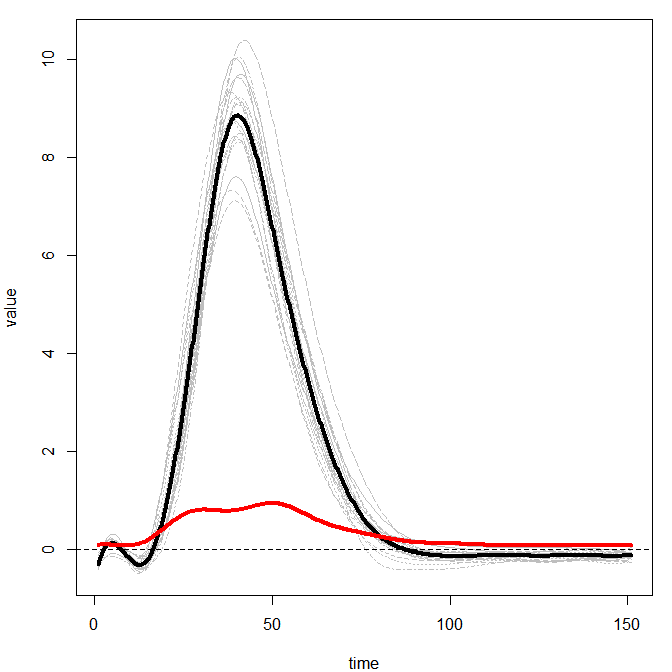
\includegraphics[height=8cm]{pinch_F_mean_var_plot.png}
    \caption{fitting pinch data using 15 b-splines: \\ Mean is black bold curve, and Sd is red bold curve.}
\end{figure}


\newpage
\subsubsection*{(c) Graph the perspective and contour plots of the sample covariance function $\hat{c}(t,s)$ of the pinch curves.}

We can easily do them by using for var.fd function of fda package and persp, contour function of R.
\begin{Rcode}
    \begin{verbatim}
pinch.F.cov <- var.fd(pinch.F)
dim(pinch.F.cov$coef) #15*15
grid <- 1:15
pinch.F.cov.mat = eval.bifd(grid, grid, pinch.F.cov)
par(mfrow=c(1,2), mar=c(4,4,1,1))
persp(grid, grid, pinch.F.cov.mat, xlab="s", ylab="t", zlab="cov(s,t)")
contour(grid, grid, pinch.F.cov.mat)
    \end{verbatim}
\end{Rcode}

Result plots are here.

\begin{figure}[hh]
    \centering
    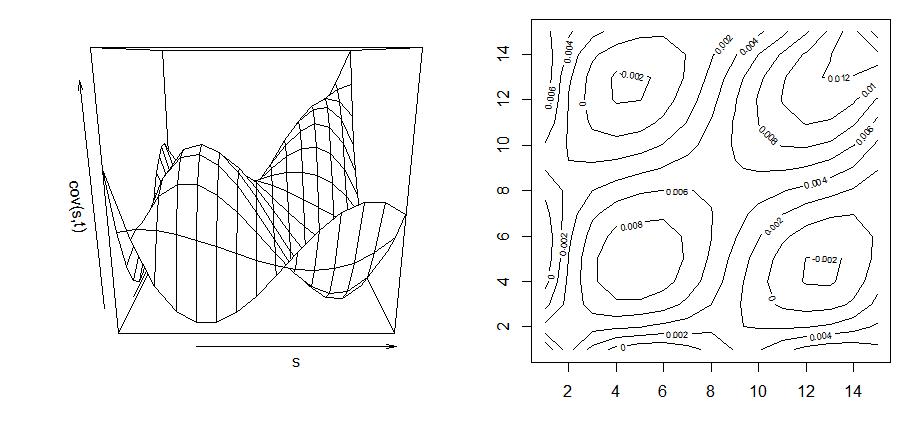
\includegraphics[height=8cm]{pinch_F_cov_persp_contour_plot.png}
    \caption{fitting pinch data using 15 b-splines: \\ covariance perspective plot and contour plot.}
\end{figure}

\newpage
\subsubsection*{(d) Graph the first four EFPC’s of the pinch data. How many components do you need to explain 90\% of variation?}

Let's do PCA with 4 components following the instruction of problem, and see the proportions of variance of each component for determining number of components for 90\% explanation.

\begin{Rcode}
    \begin{verbatim}
par(mfrow=c(1,1))
pinch.F.pca = pca.fd(pinch.F, nharm=4)
plot(pinch.F.pca$harmonics, lwd=3)
pinch.F.pca$varprop
    \end{verbatim}
\end{Rcode}

Firstly, Plot the first 4 eigenfunctions.

\begin{figure}[hh]
    \centering
    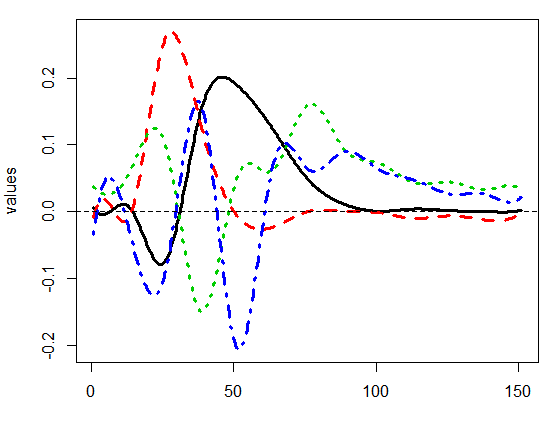
\includegraphics[height=8cm]{pinch_F_pca_4components_plot.png}
    \caption{fitting pinch data using 15 b-splines and do PCA: \\ first 4 components.}
\end{figure}

And the ouput of last line is

\begin{console}
    \begin{verbatim}
> pinch.F.pca$varprop
[1] 0.67225632 0.24845297 0.04603548 0.01933904
    \end{verbatim}
\end{console}

Since the sum of first 2 proportion is 0.9207093, we need only 2 components to reach 90\% level of explanation of variation .


\end{document}


